% ============================================================================
% Multi-Pathology Point-of-Care Diagnostic Panel Optimisation:
% A Computational Framework for the SISTER ACT Trial Context
% ============================================================================

\documentclass[11pt, oneside]{article}
\usepackage[margin=1in]{geometry}
\usepackage{authblk}
\providecommand{\leadauthor}[1]{}
\providecommand{\shorttitle}[1]{}
\renewcommand\Affilfont{\small}

\usepackage{amsmath,amssymb}
\usepackage{booktabs}
\usepackage{graphicx}
\usepackage[colorlinks=false,pdfborder={0 0 0},breaklinks=true]{hyperref}
\usepackage[capitalise,noabbrev]{cleveref}
\usepackage{microtype}
\usepackage{textcomp}
\usepackage{array}

\makeatletter
\@ifundefined{acknowledgements}{%
  \newenvironment{acknowledgements}{\section*{Acknowledgements}}{}
}{}
\@ifundefined{endkeywords}{%
  \newenvironment{keywords}{\noindent\textbf{Keywords:} }{\par}%
}{}
\makeatother

\leadauthor{Erzurumluoğlu}

\begin{document}

\title{Multi-Pathology Point-of-Care Diagnostic Panel Optimisation:\\A Computational Framework for Acute Chest Pain Triage}
\shorttitle{POCT Panel Optimisation: PACE}

\author{Roy Erzurumluoğlu\thanks{Corresponding author: \href{mailto:roy.erzurumluoglu@gmail.com}{roy.erzurumluoglu@gmail.com}}$^{,}$\thanks{ORCID: \href{https://orcid.org/0009-0000-9523-881X}{0009-0000-9523-881X}}\\
  Independent Researcher, Maastricht, The Netherlands.}

\maketitle

\begin{abstract}
When a patient walks into a Dutch GP practice with acute chest pain, the clinician has roughly fifteen minutes and a single capillary blood draw to decide: emergency referral or safe discharge? Six life-threatening diagnoses must be considered simultaneously, yet every existing decision tool (HEART, Wells, Marburg) screens for only one at a time. No framework asks the joint question: what is the minimum set of point-of-care tests that covers them all?

This paper builds one. Formalising multi-pathology panel selection as a weighted set-cover problem, the framework identifies a unique four-test panel (hs-cTnI, D-dimer, NT-proBNP, CRP) covering 5/6 pathologies with per-pathology NPV~$> 0.99$. The sixth pathology (pneumothorax) is structurally invisible to blood biomarkers. The core panel requires only a benchtop analyser and a capillary blood draw, making it deployable in both GP practices and, with a low-cost home testing device analogous to a consumer blood-pressure monitor, in patient households. Because much of the specificity data does not yet exist, a parametric sensitivity analysis propagates all uncertain inputs through the full model (2{,}000 joint Monte~Carlo draws). The result: panel selection is \textbf{invariant} to specificity uncertainty, the ED false-positive rate is bounded to 14.8 to 16.4\% (95\% credible interval) after mitigation, and the economic direction remains favourable in every draw. A second contribution is a structured evidence-gap audit: of the 82 model inputs without direct literature support, a tornado analysis identifies exactly which measurements would most reduce output uncertainty (CRP and NT-proBNP specificity for aortic dissection top the list), offering a prioritised measurement agenda for prospective trials such as SISTER~ACT. The framework is offered as a tool for trial design: the computational machinery is in place, ready to be updated as prospective data become available.
\end{abstract}

\begin{keywords}
set cover | diagnostic panel | point-of-care testing | chest pain | sensitivity analysis | biomarker | primary care | PACE
\end{keywords}

\noindent\textbf{Corresponding author:} \href{mailto:roy.erzurumluoglu@gmail.com}{roy.erzurumluoglu@gmail.com}

\newpage
\raggedbottom
\sloppy

% Aggressive float placement
\renewcommand{\dbltopfraction}{0.9}
\renewcommand{\textfraction}{0.07}
\renewcommand{\dblfloatpagefraction}{0.7}
\setcounter{dbltopnumber}{2}
\setcounter{topnumber}{3}
\setcounter{totalnumber}{5}


% ============================================================================
\section{Introduction}
\label{sec:introduction}
% ============================================================================

Primary care clinicians evaluating acute chest pain face a combinatorial diagnostic challenge: they must simultaneously exclude acute coronary syndrome (ACS), pulmonary embolism (PE), aortic dissection, pericarditis/myocarditis, tension pneumothorax, and acute heart failure using a single capillary blood sample, a benchtop analyser, and $\leq$15 minutes before a disposition decision. Current clinical decision rules (HEART + hs-cTnI~\cite{Backus2013,Schols2019,Willemsen2021}, Marburg Heart Score~\cite{Schols2018}, Wells + D-dimer~\cite{Geersing2012}) each address a \emph{single} diagnostic axis, leaving the majority of pathologies unscreened.

The parallel to combination therapy design in oncology is surprisingly close: there, one selects the minimum set of drugs whose targets collectively hit all viability-sustaining pathways~\cite{VeraLicona2013,Erzurumluoglu2026ALIN}; here, one selects the minimum set of biomarkers whose sensitivities collectively cover all target pathologies above a clinical threshold. Both reduce to the minimum hitting set problem, a classical NP-hard combinatorial optimisation~\cite{Chvatal1979}.

No existing framework treats multi-pathology POCT coverage as a joint optimisation problem. Each decision rule was developed, validated, and deployed in isolation, including recent Dutch primary care evaluations combining point-of-care troponin with modified HEART scores~\cite{Willemsen2021}. The result is a patchwork of single-axis tools with no mechanism for jointly evaluating coverage, cost, turnaround time, false-positive burden, or operational feasibility across the full threat spectrum.

\textbf{This paper tries to answer four questions:}
\begin{enumerate}
\item Can multi-pathology panel selection be formalised as a transparent, reproducible optimisation?
\item What can such a framework already tell us from currently available evidence?
\item How robust are the conclusions when we honestly propagate what we do not know?
\item Which measurements might be most valuable for a prospective trial to consider first?
\end{enumerate}


% ============================================================================
\section{Methods}
\label{sec:methods}
% ============================================================================

The framework chains seven analytical layers, each building on the last. Every input is explicitly declared, every output is reproducible, and the entire pipeline runs end-to-end from a single command.

\subsection{Coverage matrix and set-cover optimisation}

I define a coverage matrix $\mathbf{M} \in [0,1]^{6 \times 8}$ where rows are pathologies $\mathcal{P} = \{$ACS, PE, Aortic Dissection, Pericarditis/Myocarditis, Pneumothorax, Acute Heart Failure$\}$ and columns are candidate biomarkers $\mathcal{B} = \{$hs-cTnI, D-dimer, NT-proBNP, CRP, Copeptin, H-FABP, Myoglobin, Procalcitonin$\}$. All eight were selected because validated or near-market POC assays exist for capillary blood (e.g., Siemens Atellica VTLi, Roche cobas h232, immunoturbidimetric CRP cartridges). Entry $M_{p,b}$ is the pooled diagnostic sensitivity of biomarker $b$ for pathology $p$, with 95\% confidence intervals. Of the 48 entries, 30 (63\%) derive from published meta-analyses or diagnostic accuracy studies~\cite{Lipinski2015,Geersing2012,Maisel2002,Nazerian2014,Keller2011,Raskovalova2013,Body2015,Imazio2011,Crawford2019}; the remaining 18 are non-viable combinations set to zero.

A biomarker $b$ \emph{covers} pathology $p$ at threshold $\tau$ if $M_{p,b} \geq \tau$. The panel selection problem minimises:
\begin{equation}
\min_{\mathbf{x}} \sum_{b \in \mathcal{B}} \Big[ w_{\text{size}} + w_{\text{cost}} \cdot c_b + w_{\text{time}} \cdot t_b + w_{\text{sample}} \cdot v_b \Big] \cdot x_b
\label{eq:objective}
\end{equation}
subject to coverage constraints:
\begin{equation}
\sum_{b \in \mathcal{B}} a_{p,b} \cdot x_b \geq 1 \quad \forall\, p \in \mathcal{P}^*
\label{eq:coverage}
\end{equation}
where $\mathcal{P}^*$ is the set of coverable pathologies and $x_b \in \{0,1\}$. The ILP is solved via \texttt{scipy.optimize.milp} (HiGHS backend), with exhaustive enumeration of all $2^8 = 256$ subsets as verification.

\subsection{Uncertainty quantification}

Three complementary methods propagate input uncertainty:
\begin{itemize}
\item \textbf{Monte Carlo.} $n = 5{,}000$ sensitivity matrices sampled from $\text{Beta}(\alpha, \beta)$ fitted to published CIs; coverage, detections, and net benefit recomputed for the fixed optimal panel.
\item \textbf{Bootstrap stability.} $n = 1{,}000$ iterations: sample sensitivities, re-solve ILP, record panel composition and validity.
\item \textbf{Parametric sensitivity analysis.} All clinical estimates (specificity, QALY losses, and other uncertain parameters) are assigned Beta priors; 2{,}000 joint Latin Hypercube draws propagated through the full false-positive cascade and economic model (\cref{sec:sensitivity_analysis}).
\end{itemize}

\subsection{False-positive cascade and copula correction}

A multi-analyte rule-out panel at low prevalence will generate false positives. The framework computes the false-positive rate at four interpretation layers: (1)~binary OR (any positive $\to$ referral), (2)~Gaussian copula correction for biomarker correlation~\cite{Nelsen2006}, (3)~quantitative likelihood-ratio interpretation per pathology, and (4)~pathology-directed management routing (pericarditis/AHF $\to$ outpatient, not ED). Each layer is additive and separately auditable.

\subsection{Health-economic modelling}

A single-cycle decision tree compares three strategies (current care, optimal panel alone, full PACE composite) on cost per patient, sensitivity, missed diagnoses, and incremental cost-effectiveness ratio (ICER). QALY losses for missed diagnoses are grounded in published cost-utility analyses: AoD from Thokala~2024~\cite{Thokala2024AAS} ($\sim$1.9~QALYs), PE from Boon~2021~\cite{Boon2021CTEPH} (2.04~QALYs), ACS from Fox~2005~\cite{Fox2005} and Reed~2007~\cite{Reed2007}. Only pneumothorax lacks QALY-based CUA data.

\subsection{PACE composite score}

The framework evaluates the biomarker panel within a composite clinical decision rule integrating symptoms, signs, ECG, risk factors, timeline, and the POC panel. I call this the PACE score (Panel-Augmented Chest pain Evaluation). It is benchmarked against HEAR and HEART at matched sensitivity.

The framework is designed for two deployment settings. In GP practices, the full PACE composite (biomarker panel plus clinical decision rule) can run on existing benchtop analysers within a standard consultation. For home-based triage, the core biomarker panel could be delivered through a low-cost, self-contained testing device, analogous in form factor and price point to a consumer blood-pressure monitor, requiring only a capillary finger-prick and returning results in under 15 minutes. Both settings cover 5/6 pathologies; pneumothorax, which no blood biomarker can detect, remains the acknowledged gap.

\subsection{Implementation}

All analyses in Python 3.12 (\texttt{scipy}, \texttt{numpy}, \texttt{matplotlib}). Full code, data provenance, and results: \url{https://github.com/royerz2/PanDiagnosticCardiology}. The pipeline runs 23 steps end-to-end, generating all results, figures, and sensitivity analyses from a single command.


% ============================================================================
\section{Results}
\label{sec:results}
% ============================================================================

\subsection{The optimal panel is uniquely determined}

At $\tau = 0.90$, the ILP and exhaustive enumeration return the identical panel:

\begin{center}
\textbf{hs-cTnI + D-dimer + NT-proBNP + CRP}
\end{center}

\noindent (4 tests, 83.3\% coverage, \texteuro36, 15\,min, 55\,$\mu$L capillary blood). This solution is \textbf{unique}: each pathology has exactly one biomarker exceeding $\tau$, so the coverage constraint forces selection of all four regardless of cost weights. Across 500 random weight configurations spanning four orders of magnitude, the same panel was selected in 100\% of cases. \cref{fig:heatmap} shows the coverage matrix.

\begin{figure}[!htb]
\centering
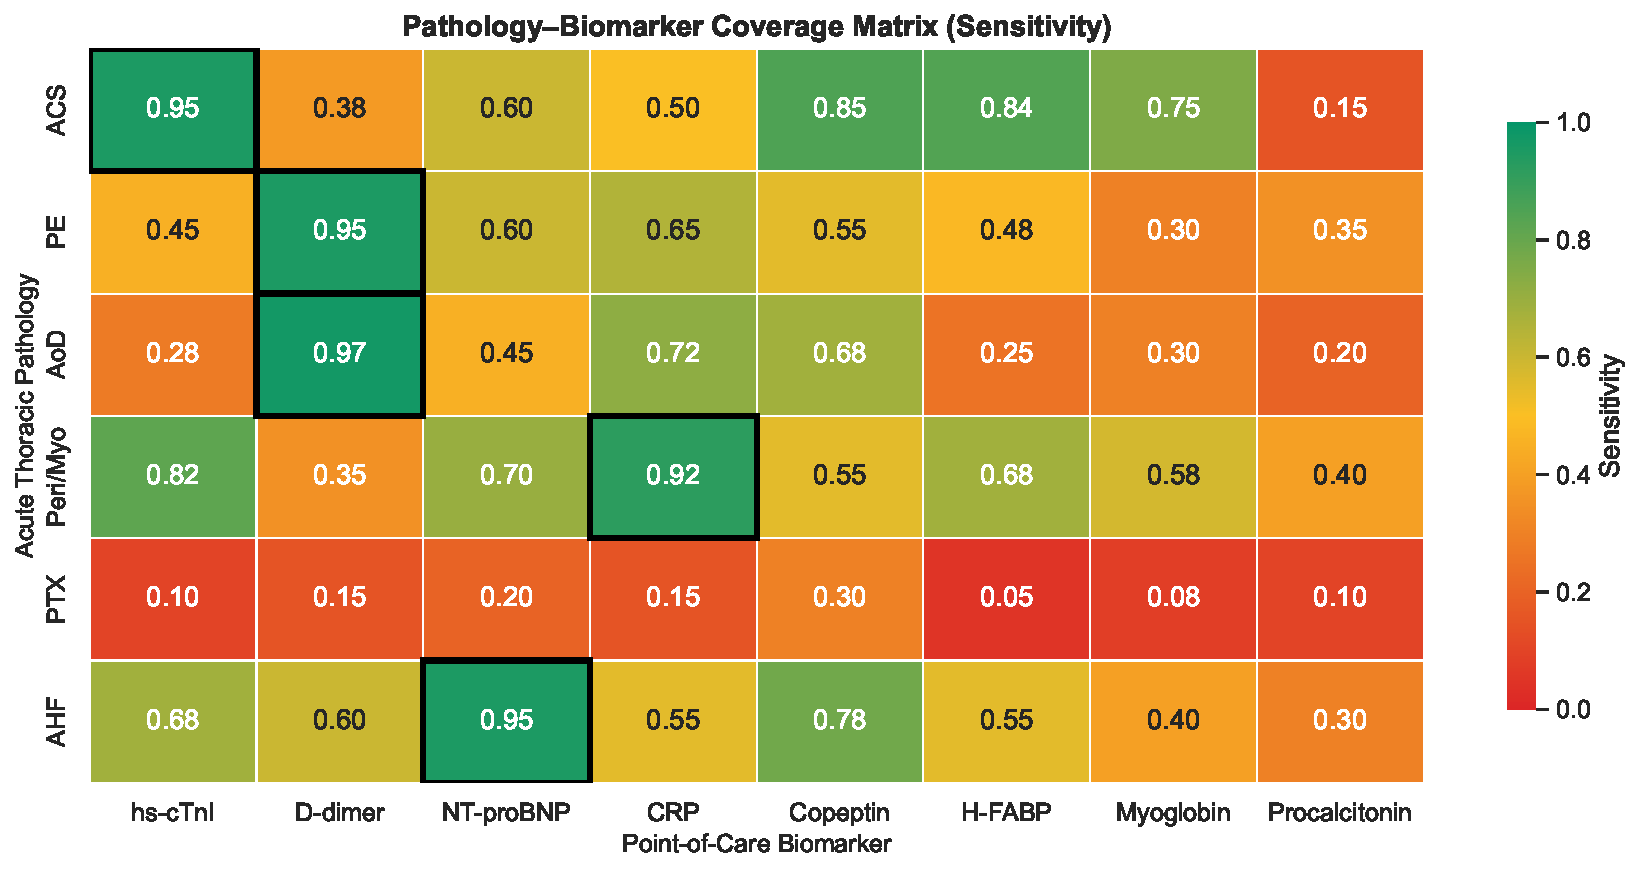
\includegraphics[width=0.85\linewidth]{../figures/fig1_coverage_heatmap}
\vspace{-6pt}
\caption{\textbf{Pathology-biomarker coverage matrix.} Each cell shows pooled meta-analytic sensitivity. The pneumothorax row is uniformly pale: no biomarker exceeds 0.30.}
\label{fig:heatmap}
\end{figure}

\subsection{Bootstrap stability: one fragile input with trial design consequences}

Bootstrap resampling ($n = 1{,}000$) selects the four-test panel in \textbf{75.6\%} of iterations. The other three biomarkers are robust: D-dimer 100\%, NT-proBNP 99.9\%, hs-cTnI 98.4\% inclusion. The fragile input is CRP sensitivity for pericarditis (point estimate 0.92, P(sampled $< \tau$) = 20.5\%).

This is arguably the single most practically important result for trial design. When CRP drops below the 0.90 threshold, the solver falls back to a three-test panel (hs-cTnI, D-dimer, NT-proBNP) covering four pathologies. Pericarditis and myocarditis lose their rule-out biomarker entirely, and the clinical product changes from a five-pathology screen to a four-pathology one. A one-in-five chance of this degradation is too high to accept without resolution.

Two remediation paths merit prospective evaluation. First, copeptin: the framework's threshold analysis shows that if copeptin achieves $\geq$0.90 sensitivity for pericarditis, it would enter the panel as a CRP backup, restoring five-pathology coverage regardless of the CRP value. Second, serial CRP: an elevated CRP drawn at 0 and 6 hours might improve diagnostic confidence for pericarditis, analogous to the serial troponin protocol for ACS. Either pathway would need to be evaluated in the first phase of a trial such as SISTER ACT, before the four-test panel can be considered stable.

\subsection{Clinical utility}

\cref{tab:utility} reports the clinical utility of the optimal panel. All five covered pathologies achieve NPV $> 0.99$, confirming individual rule-out suitability~\cite{Lord2006}.

\begin{table}[h]
\centering
\caption{Clinical utility of the optimal panel.}
\label{tab:utility}
\scriptsize
\setlength{\tabcolsep}{3pt}
\begin{tabular}{@{}llcccccl@{}}
\toprule
\textbf{Path.} & \textbf{Marker} & \textbf{Se} & \textbf{Sp} & \textbf{Prev} & \textbf{NPV} & \textbf{PPV} & \textbf{RO} \\
\midrule
ACS  & hs-cTnI   & .95 & .54 & 3.5\% & .997  & .070 & $\checkmark$ \\
PE   & D-dimer   & .95 & .42 & 1.5\% & .998  & .024 & $\checkmark$ \\
AoD  & D-dimer   & .97 & .47 & 0.3\% & $>$.999 & .005 & $\checkmark$ \\
Peri & CRP       & .92 & .38 & 4.0\% & .991  & .058 & $\checkmark$ \\
AHF  & NT-proBNP & .95 & .76 & 2.5\% & .998  & .092 & $\checkmark$ \\
PTX  & (none)    & .20$^*$ & - & 0.5\% & -   & -  & $\times$ \\
\bottomrule
\end{tabular}
\par\noindent{\scriptsize RO = rule-out suitable. $^*$Best-Se marker in panel (NT-proBNP, 0.20); not rule-out suitable. $^\dagger$No biomarker covers pneumothorax; clinical auscultation remains the primary bedside detection method.}
\end{table}

\subsection{False-positive cascade: point estimates}

\cref{tab:fp_cascade} presents the false-positive mitigation cascade.

\begin{table}[h]
\centering
\caption{False-positive mitigation cascade for the optimal panel.}
\label{tab:fp_cascade}
\scriptsize
\setlength{\tabcolsep}{3pt}
\begin{tabular}{@{}lcc@{}}
\toprule
\textbf{Interpretation layer} & \textbf{FP rate} & \textbf{Discharge} \\
\midrule
Binary OR (any pos.\ $\to$ ED) & 93.4\% & 6.6\% \\
+ Copula correction & 86.5\% & 13.5\% \\
+ Quantitative LR (per-path.\ thresholds) & 66.8\%$^a$ & 33.2\% \\
+ Path.-directed routing$^b$ & 63.3\%$^c$ & 33.2\% \\
+ HEAR pre-stratification (test 35\%) & 37.2\%$^d$ & - \\
\bottomrule
\end{tabular}
\par\noindent{\scriptsize $^a$Any-pathology FP (copula). $^b$Peri/AHF $\to$ outpatient. $^c$ED-only FP. $^d$Per 1000 presentations.}
\end{table}

\noindent Pneumothorax does not contribute to the false-positive cascade because no biomarker covers it. In clinical practice, auscultation (absent breath sounds) remains the standard bedside screen; the biomarker panel therefore complements, rather than replaces, routine physical examination.

The key transition is from binary cutoffs to quantitative likelihood-ratio interpretation: a mildly elevated D-dimer no longer triggers the same referral as a markedly elevated one. Combined with pathology-directed routing and HEAR pre-stratification, the framework yields 372 unnecessary ED referrals per 1000 presentations, a 22.0\% reduction versus binary interpretation.

\subsection{PACE composite score}

When the biomarker panel is embedded in the full composite clinical decision rule, the modelled system achieves \textbf{97.7\% sensitivity} and \textbf{70.0\% specificity} across all six pathologies, with a referral rate of 38.2\% and NPV of 99.6\%. For comparison: HEAR achieves 42.4\% specificity (referral 62.2\%) and HEART achieves 49.3\% specificity (referral 56.4\%) at comparable sensitivity.

\subsection{Health economics: model structure, not point estimates}

A single-cycle decision tree compares three strategies (current care, optimal panel alone, full PACE composite) across cost per patient, sensitivity, missed diagnoses, and QALYs gained. QALY losses for missed diagnoses are grounded in published cost-utility analyses where available (AoD, PE, ACS) and estimated where not. In all three pairwise comparisons and across all 2{,}000 sensitivity analysis draws, the panel-based strategies dominate current care: they improve outcomes while reducing net cost, primarily by averting downstream expenditure from missed diagnoses.

However, the absolute ICER values span a wide range depending on input assumptions, and the single-cycle structure omits long-term cost trajectories that a full Markov model would capture. I therefore report the \emph{direction} (dominant in every draw) but not the specific magnitudes, which should not be taken at face value. The model structure is sound and ready to accept patient-level cost and outcome data from a prospective study; the numbers it currently produces are illustrative, not actionable.

\subsection{Parametric sensitivity analysis: what if the estimates are wrong?}
\label{sec:sensitivity_analysis}

The results above rely on \emph{point estimates} for parameters that I could not ground in published diagnostic accuracy data: specificities for non-primary pathologies and other clinical estimates. I do not want to pretend these are known. Instead, I treat them as genuinely uncertain, assigning each a Beta prior and propagating them jointly, to find out whether the conclusions hold up and, if they wobble, which unknowns are responsible.

\textbf{Method.} Each uncertain parameter is assigned a $\text{Beta}(\alpha, \beta)$ prior fitted via method-of-moments from the plausible range (point estimate $\pm$ clinical uncertainty). From 2{,}000 joint Monte Carlo draws (Latin Hypercube sampling), each draw generates a full specificity override vector; the complete false-positive cascade (copula with 20{,}000 samples, quantitative LR, pathology-directed routing) and simplified ICER are recomputed for every draw.

\textbf{Result 1: Panel selection is invariant.} In 100\% of 2{,}000 draws, the ILP returns the same four-test panel. Panel composition is determined by sensitivity data (which is literature-grounded); no plausible variation in specificity or downstream parameters alters it.

\textbf{Result 2: 95\% credible intervals on all outputs.} \cref{tab:sa_ci} shows that even under joint uncertainty, the conclusions are bounded.

\begin{table}[h]
\centering
\caption{95\% credible intervals from parametric sensitivity analysis (2{,}000 joint draws).}
\label{tab:sa_ci}
\scriptsize
\setlength{\tabcolsep}{3pt}
\begin{tabular}{@{}lcccc@{}}
\toprule
\textbf{Metric} & \textbf{Point} & \textbf{2.5\%} & \textbf{97.5\%} & \textbf{Width} \\
\midrule
FP binary OR           & 93.5\% & 93.5\% & 93.5\% & 0.0pp \\
FP copula-corrected    & 86.6\% & 86.1\% & 87.0\% & 0.9pp \\
FP quantitative LR     & 21.8\% & 21.0\% & 22.5\% & 1.5pp \\
FP ED-only             & 15.6\% & 14.8\% & 16.4\% & 1.6pp \\
HEAR ED/1000           & 54.7   & 51.8   & 57.3   & 5.5 \\
Discharge rate         & 78.2\% & 77.5\% & 79.0\% & 1.5pp \\
\bottomrule
\end{tabular}
\par\noindent{\scriptsize pp = percentage points. Width = 97.5\% $-$ 2.5\%.}
\end{table}

The operationally critical metric, the ED false-positive rate after all mitigation, ranges from \textbf{14.8\% to 16.4\%}, a 1.6 percentage-point band. This is narrow enough to support directional conclusions even without prospective specificity data. Notably, the binary OR layer (93.5\%) is entirely deterministic: it depends only on global specificity values, which are fixed by literature data, so all output uncertainty originates in the quantitative likelihood-ratio interpretation step and the HEAR pre-stratification layer.

\textbf{Result 3: Economic direction is favourable in 100\% of draws.} No plausible combination of uncertain inputs reverses the direction; panel-based strategies dominate current care in every draw. Absolute magnitudes vary widely with input assumptions and should be treated as illustrative.

\subsection{Tornado analysis: which unknowns matter most?}

\cref{fig:tornado} shows the tornado plot from one-at-a-time sensitivity analysis on the ED false-positive rate.

\begin{figure}[!htb]
\centering
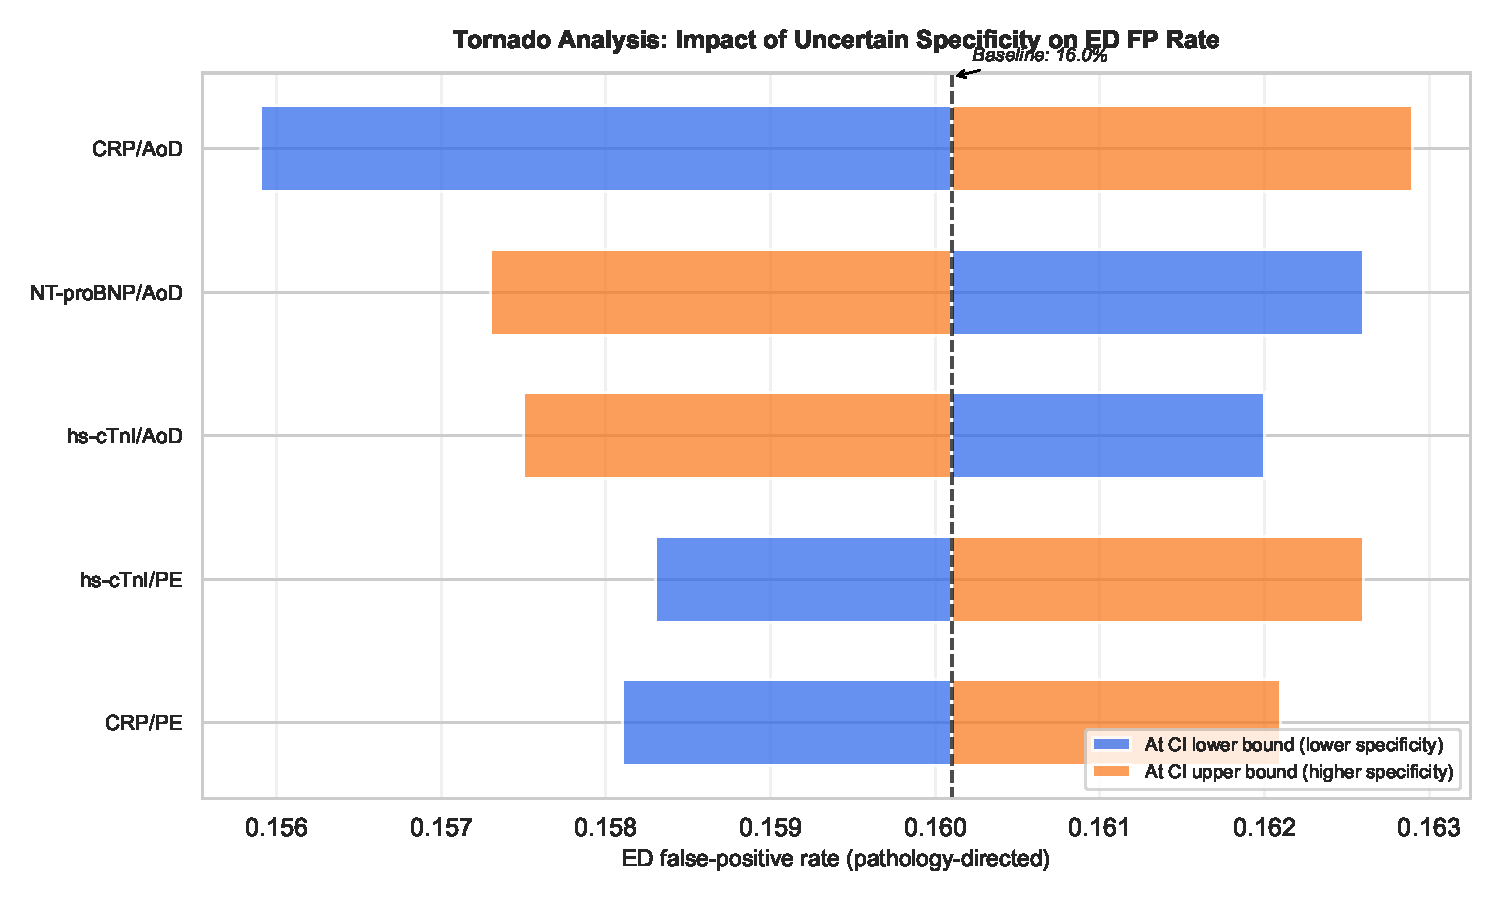
\includegraphics[width=0.85\linewidth]{../figures/fig12_tornado_sensitivity}
\vspace{-6pt}
\caption{\textbf{Tornado plot: impact of each uncertain specificity on ED false-positive rate.} Bar length = swing (difference between FP rate at CI lower bound vs.\ upper bound). CRP specificity for aortic dissection and NT-proBNP specificity for aortic dissection dominate output uncertainty.}
\label{fig:tornado}
\end{figure}

The top five drivers of output uncertainty are:
\begin{enumerate}
\item CRP specificity for AoD (swing: 0.70pp)
\item NT-proBNP specificity for AoD (swing: 0.53pp)
\item hs-cTnI specificity for AoD (swing: 0.45pp)
\item hs-cTnI specificity for PE (swing: 0.43pp)
\item CRP specificity for PE (swing: 0.40pp)
\end{enumerate}

These five parameters account for the large majority of total output uncertainty. The remaining 17 panel-relevant parameters contribute $<$0.1pp each. This suggests a clear measurement priority: \textbf{CRP and NT-proBNP specificity for aortic dissection} appear to be the two inputs whose prospective measurement would most reduce the framework's remaining uncertainty.

\subsection{What-if envelope}

\cref{fig:envelope} presents the what-if analysis.  Panel~A asks a simple question: ``What if a prospective trial measures these 16 unknown per-pathology specificities and finds they are all very low, or all very high, or especially poor for aortic dissection?''  Panel~B shows the joint posterior distribution from 2{,}000 Monte~Carlo draws where all uncertain parameters vary simultaneously.

\begin{figure}[!htb]
\centering
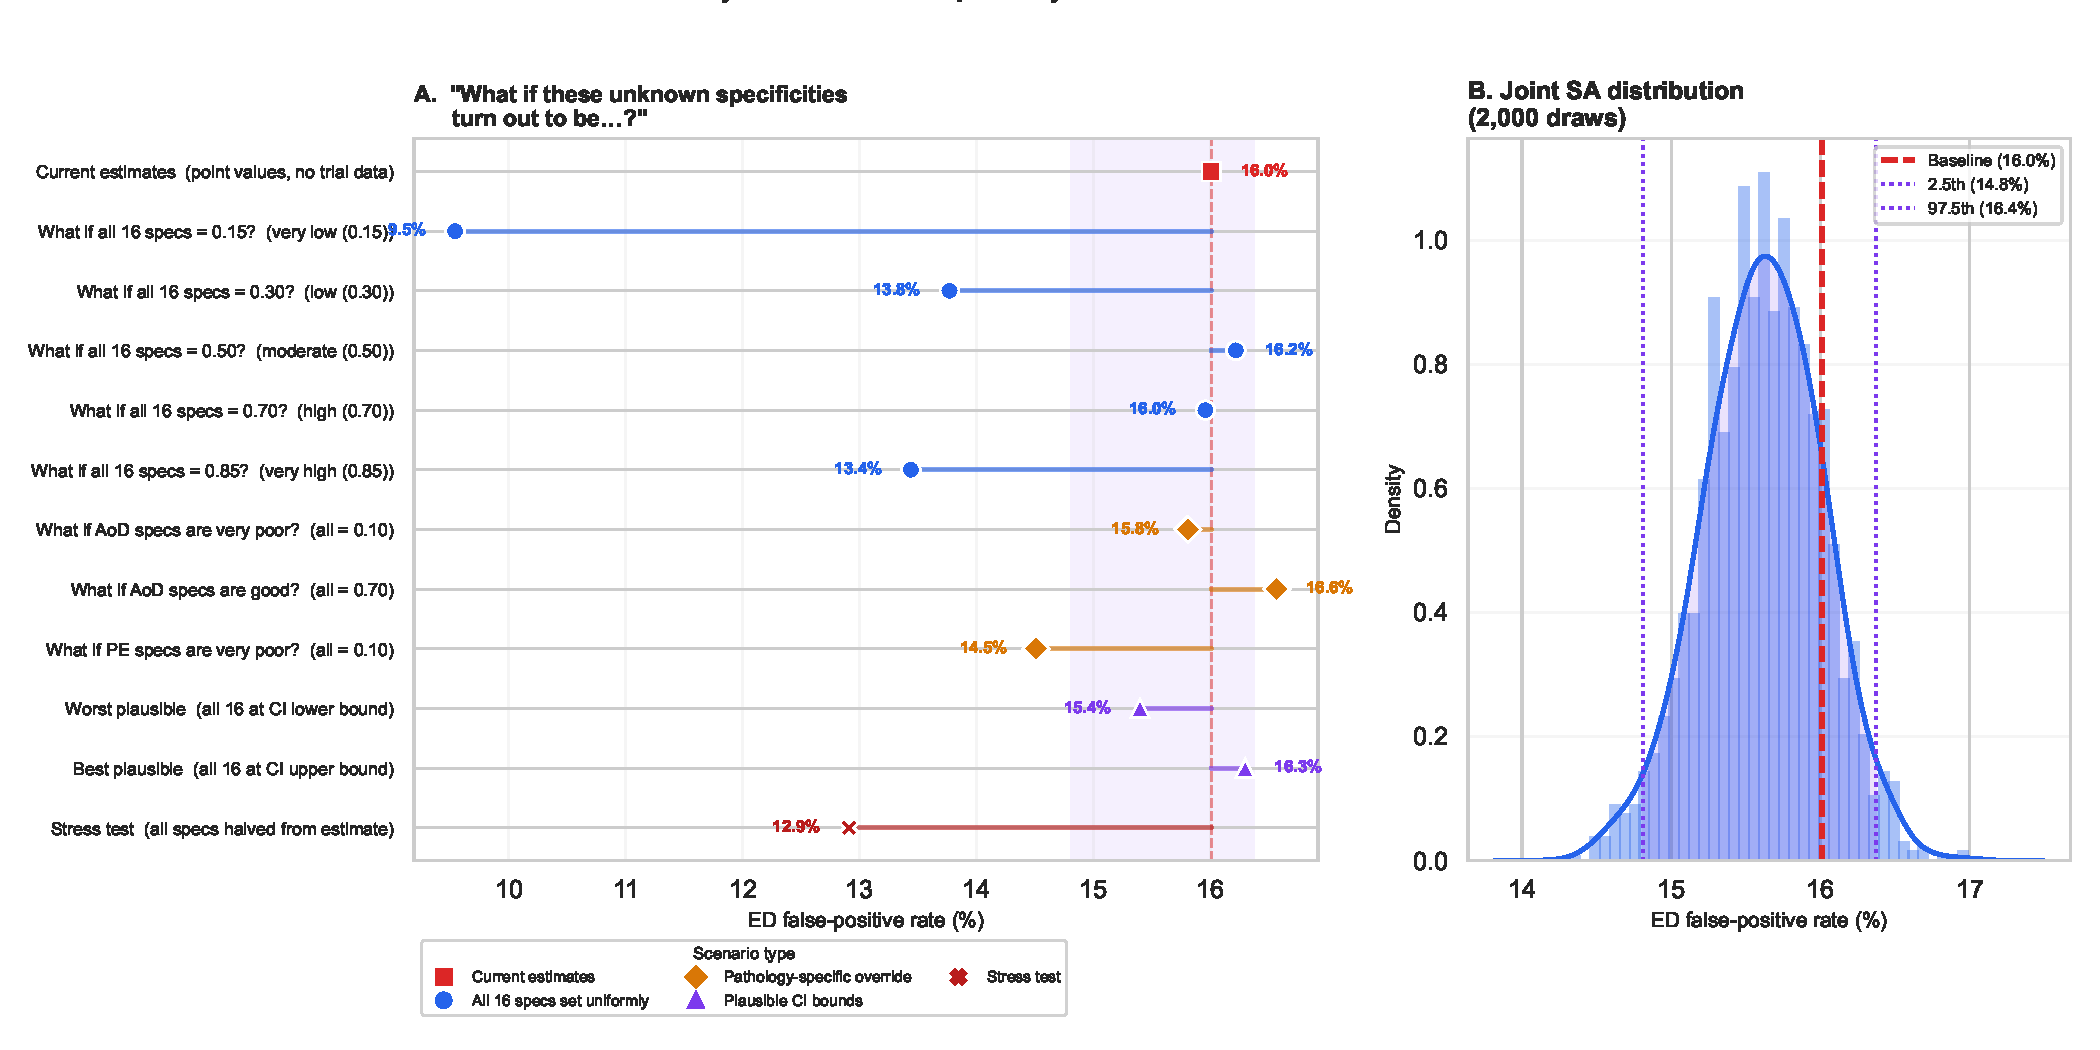
\includegraphics[width=0.95\linewidth]{../figures/fig13_whatif_envelope}
\vspace{-6pt}
\caption{\textbf{What-if analysis of unknown specificity values.}
\textbf{(A)}~Lollipop chart of 12 named scenarios, each positing a different answer to the question ``What if these 16 unknown specificities turn out to be\ldots?''
Blue dots: uniform assumptions (all 16 set to the same value);
orange diamonds: pathology-targeted overrides (aortic dissection, pulmonary embolism);
purple triangles: plausible CI bounds; red cross: stress test (all halved).
The dashed red line marks the baseline estimate (16.0\%).
Even the most extreme scenario (all specs = 0.15) yields only 9.5\% ED~FP, while
the tightest plausible range is 15.4 to 16.3\%.
\textbf{(B)}~Histogram and kernel-density estimate of 2{,}000 joint Monte~Carlo draws
with the 95\% credible interval (14.8 to 16.4\%) shaded.}
\label{fig:envelope}
\end{figure}


% ============================================================================
\section{Discussion}
\label{sec:discussion}
% ============================================================================

If the computational framework above is the engine, then prospective clinical data is the fuel it currently lacks. A systematic audit of the model's inputs identified 82 values without direct literature support (specificities, correlations, and economic parameters) that I estimated from clinical reasoning and indirect evidence. Making this gap structure explicit, rather than burying it in a limitations paragraph, is itself a contribution: it converts an unavoidable weakness into a prioritised measurement agenda. \cref{tab:gaps} summarises the seven principal evidence gaps, ranked by their estimated impact on framework uncertainty as determined by the tornado analysis and bootstrap results.

\begin{table}[h]
\centering
\caption{Prioritised evidence-gap audit: knowledge gaps ranked by impact on framework uncertainty.}
\label{tab:gaps}
\scriptsize
\setlength{\tabcolsep}{3pt}
\begin{tabular}{@{}clp{5.2cm}cc@{}}
\toprule
\textbf{\#} & \textbf{Gap} & \textbf{Why it matters} & \textbf{\# unknowns} & \textbf{Priority} \\
\midrule
1 & Biomarker specificity & 34/48 specificity entries are clinical estimates; top two tornado drivers (CRP and NT-proBNP spec.\ for AoD) sit here & 34 & Critical \\
2 & CRP sensitivity (pericarditis) & Single fragile sensitivity input: panel drops to 3 tests in 20.5\% of bootstrap iterations & 1 & High \\
3 & Early-presenter troponin timing & hs-cTnI sensitivity drops to $\sim$0.70 at $<$3\,h; copeptin may restore coverage without serial draws & 1 & High \\
4 & Pneumothorax detection & No biomarker exceeds 0.30 sensitivity; structural gap requiring non-blood modality & 0 & Moderate \\
5 & HEAR score validation & Not validated in Dutch primary care; affects FP estimates for 35\% moderate-risk stratum & 1 & Moderate \\
6 & Health-economic inputs & Single-cycle decision tree with estimated costs; directional signal only & $\sim$12 & Low \\
7 & Spectrum bias (ED $\to$ GP) & All sensitivity data from ED cohorts; Dutch primary care may have systematically lower values due to earlier, milder presentations & 30+ & High \\
\bottomrule
\end{tabular}
\par\noindent{\scriptsize Priority reflects estimated impact on framework conclusions from tornado analysis, bootstrap stability, and sensitivity analysis. \# unknowns = count of model inputs without direct literature support in this category.}
\end{table}

\subsection{Gap~1: Biomarker specificity in primary care}

The specificity matrix (8 biomarkers across 6 pathologies) relies on clinical estimates for 34 of its 48 entries. This is the largest single source of uncertainty in the framework. The tornado analysis (\cref{fig:tornado}) identifies CRP specificity for aortic dissection and NT-proBNP specificity for aortic dissection as the two parameters whose measurement would most reduce output uncertainty.

A prospective cohort study nested within SISTER ACT, collecting all 8 biomarker values alongside final diagnoses in chest pain presentations, could simultaneously fill all 34 specificity gaps and the 16 pairwise correlations used in the copula model. The framework would then re-run automatically with no methodological changes, just updated numbers.

\subsection{Gap~2: CRP sensitivity for pericarditis}

The bootstrap analysis flags CRP for pericarditis as the single fragile sensitivity input: in 20.5\% of resampled iterations, CRP's sensitivity falls below the 0.90 threshold and the panel drops to three tests covering four pathologies. Confirming (or refuting) this value prospectively would either validate the four-test panel or immediately highlight the coverage gap so that alternatives can be evaluated.

\subsection{Gap~3: Early presenters and troponin timing}

At less than three hours post-symptom onset, hs-cTnI sensitivity drops from 0.95 to roughly 0.70, below the coverage threshold. The ESC 0/1-hour serial troponin algorithm~\cite{Collet2021}, recently shown feasible in emergency primary care~\cite{Johannessen2025}, could recover ACS coverage but requires timed serial draws. An alternative worth exploring is copeptin: the framework's threshold analysis suggests that if copeptin ACS sensitivity reaches 0.90 (as indicated by dual-marker studies~\cite{Raskovalova2013,Mu2023,Giannitsis2021}), it would enter the panel and restore full coverage without serial testing.

\subsection{Gap~4: Pneumothorax detection}

No candidate biomarker exceeds 0.30 sensitivity for pneumothorax. This is a structural gap that no blood-based marker is likely to fix. The panel covers 5/6 pathologies; pneumothorax remains the acknowledged limitation, requiring clinical assessment or future non-blood modalities for detection.

\subsection{Gap~5: HEAR score in Dutch primary care}

The HEAR pre-stratification step limits panel testing to the $\sim$35\% of patients in the moderate-risk stratum, substantially reducing unnecessary referrals. However, HEAR has not been prospectively validated in Dutch primary care~\cite{VandenBulk2024}. If its risk stratification performs differently in this population, the downstream false-positive estimates would shift. Validating HEAR in this setting, already a stated SISTER ACT objective, would anchor one of the framework's key operational assumptions.

\subsection{Gap~6: Health-economic inputs}

The health-economic analysis consistently produces dominant ICERs: the panel saves money and improves outcomes, and the sensitivity analysis confirms this direction across all 2{,}000 draws. But the underlying model is a single-cycle decision tree with estimated inputs. It gives a directional signal, not a definitive answer. A full Markov model built on patient-level cost and outcome data would be needed to make credible economic claims. The framework's economic module is designed to accept this data when it becomes available.

\subsection{Gap~7: Spectrum bias --- from ED to primary care}

Nearly all published sensitivity data used in the coverage matrix derive from emergency department cohorts. In the Dutch healthcare system, GP gatekeeping means that primary care chest pain presentations are systematically earlier post-symptom onset, lower acuity, and narrower in disease spectrum than ED populations. This rightward shift along the disease severity axis is expected to reduce diagnostic sensitivity: milder cases produce lower biomarker concentrations, pushing more true positives below assay cutoffs.

The magnitude of this effect is clinically consequential. If primary care sensitivities are even 5 percentage points lower than the ED-derived values, CRP for pericarditis drops from 0.92 to 0.87, well below the 0.90 coverage threshold, and the panel loses pericarditis coverage entirely. At a 10-point reduction, hs-cTnI for ACS falls from 0.95 to 0.85 and approaches the threshold boundary. The framework can be re-run with any downward-adjusted sensitivity vector; the bootstrap and Monte Carlo machinery will automatically propagate the consequences.

I propose that the first 300 SISTER ACT inclusions be used to compute primary-care-specific sensitivity estimates for at least the four panel markers. If these estimates confirm ED-derived values (within confidence intervals), the framework's current conclusions hold. If they reveal systematic attenuation, the ILP will re-solve with updated inputs and may identify a different optimal panel, possibly including copeptin or H-FABP as replacements. This is exactly the scenario for which the framework was designed: a structured tool that updates its conclusions when better data arrive.

\subsection{Trial design implications: from tornado plot to data collection protocol}

The tornado analysis and bootstrap results translate directly into concrete priorities for the SISTER ACT data collection protocol. Three recommendations follow from the computational results:

\textbf{Priority 1: Resolve the top two tornado drivers.} The framework suggests collecting all 8 candidate biomarker values in parallel with final diagnoses in the first 300 inclusions, specifically to resolve CRP and NT-proBNP specificity for aortic dissection, the two parameters that together account for the majority of output uncertainty. A case report form (CRF) designed to capture per-pathology biomarker values (not just the four panel markers) would simultaneously fill all 34 specificity gaps and the 16 pairwise correlations used in the copula model.

\textbf{Priority 2: Confirm or refute CRP sensitivity for pericarditis.} The 20.5\% bootstrap failure rate for this single input determines whether the clinical product is a five-pathology or four-pathology screen. The first interim analysis (e.g., after 150 inclusions) should include a point estimate and confidence interval for this value. If CRP sensitivity falls below 0.90, copeptin should be evaluated as a replacement marker.

\textbf{Priority 3: Anchor the HEAR score in Dutch primary care.} The HEAR pre-stratification step is not yet validated in this population. Standard operating procedures (SOPs) for the trial should include systematic HEAR scoring alongside the biomarker panel from day one, so that HEAR's stratification performance can be assessed as a secondary endpoint without requiring a protocol amendment.

These priorities are not hypothetical; they concern the design of forms, standard operating procedures, and interim analysis plans --- the practical infrastructure that determines whether a trial produces the data a framework like this one needs.

\subsection{A tool, not a prescription}

I want to be clear about what this framework is and what it is not. It is not a clinical guideline, and it does not presume to tell anyone what to do. It is a structured analytical tool, one that takes explicitly stated inputs, runs them through a reproducible pipeline, and returns quantified outputs with honest uncertainty bounds. Every cell in the coverage matrix, every specificity estimate, every economic parameter can be updated as prospective data become available; the framework will automatically propagate those changes through all 23 analytical steps and return revised conclusions.

My hope is that this might be useful: as a starting point for trial design discussions, as a way to identify which measurements would be most informative, or simply as a transparent record of one researcher's attempt to think through the multi-pathology panel selection problem systematically. The tornado plot suggests where measurement effort might begin; the sensitivity analysis shows how much (or how little) the answers depend on what we do not yet know. The rest is for the research team to decide.


\subsection{What the sensitivity analysis changes}

The sensitivity analysis changes what this paper can honestly claim. Without it, the framework would present point estimates built partly on clinical reasoning, and the reader would have to take them on faith. With it, the framework can say something more useful: ``\emph{here is the range of conclusions consistent with everything we do not yet know, and here is exactly which measurements would most narrow that range.}'' In practical terms:

\begin{enumerate}
\item The optimal panel is determined by sensitivity data (which is literature-grounded) and is completely invariant to specificity uncertainty.
\item The ED false-positive rate after all mitigation is bounded to 14.8 to 16.4\% (95\% CI), a 1.6pp band that is narrow enough for operational planning.
\item The economic direction is favourable in 100\% of draws; even the worst-case uncertain inputs do not reverse it. Absolute magnitudes are illustrative only.
\item Two parameters (CRP specificity for AoD and NT-proBNP specificity for AoD) appear to drive most of the remaining uncertainty, suggesting they may be the highest-value measurement targets.
\end{enumerate}

\subsection{Transparency, not computational power}

With only 8 biomarkers ($2^8 = 256$ subsets), there is nothing computationally impressive here: any laptop can enumerate all combinations in seconds. The contribution, if there is one, is methodological: a transparent, reproducible formulation that makes panel selection auditable. The ILP objective (\cref{eq:objective}), coverage constraints (\cref{eq:coverage}), and all input data are fully specified, enabling any reader to verify or challenge the result. The framework's value scales with candidate pool size: at 12+ biomarkers, exhaustive enumeration becomes impractical and the ILP formulation becomes necessary. An extended 12-biomarker analysis (adding sST2, GDF-15, Galectin-3, MR-proADM~\cite{Dieplinger2015,Januzzi2016,Kempf2007,Wollert2017,deBoer2012,Nishida2008,Maisel2010}) confirms the optimal panel is unchanged at $\tau = 0.90$.

\subsection{From worst-case FP to operational reality}

The 93.4\% panel-level FP rate under binary interpretation is a mathematical worst case that describes an interpretation protocol no one should use. The mitigation cascade reduces this to 63.3\% at the ED-specific level (copula-corrected) and to 372 per 1000 presentations after HEAR pre-stratification. The sensitivity analysis bounds the ED-only rate to 14.8 to 16.4\% after full mitigation, demonstrating that even with uncertain specificity inputs, the operational FP burden is manageable.

Sequential testing provides further operational mitigation: Bayesian information-theoretic test ordering reduces mean tests per patient from 4 to 2.6, reducing both cost and cumulative false-positive exposure.

When embedded in the PACE composite score, the modelled system reaches 70.0\% specificity at 97.7\% sensitivity, a notable improvement over HEAR (42.4\%) or HEART (49.3\%) at comparable sensitivity, though these numbers await prospective validation.

\subsection{Limitations}

\begin{enumerate}
\item \textbf{Data provenance}: Of 48 core sensitivity values, 30 are literature-sourced; 18 are set to zero. For specificity, correlations, and extended biomarkers, 82 values are clinical estimates. The sensitivity analysis addresses this directly by propagating all uncertain inputs.
\item \textbf{CRP fragility}: CRP for pericarditis is the single fragile sensitivity input (P(sampled $< \tau$) = 20.5\%).
\item \textbf{Single-cycle economics}: The health-economic model is directional, not definitive.
\item \textbf{Conditional independence}: Sequential testing assumes conditional independence given disease status.
\item \textbf{SA absolute values}: The sensitivity analysis computes \emph{relative} parameter impact via a standalone false-positive model; absolute FP numbers for clinical planning should come from the full pipeline's 200{,}000-sample copula simulation.
\end{enumerate}


% ============================================================================
\section{Conclusion}
\label{sec:conclusion}
% ============================================================================

This work formalises multi-pathology point-of-care diagnostic panel selection as a weighted set-cover problem and applies the resulting framework to the SISTER ACT clinical context: acute chest pain triage in Dutch primary care. At $\tau = 0.90$, the uniquely optimal panel is hs-cTnI, D-dimer, NT-proBNP, and CRP, covering 5/6 life-threatening thoracic pathologies with per-pathology NPV $> 0.99$. The sixth (pneumothorax) is structurally invisible to blood biomarkers and remains the acknowledged coverage gap. The core biomarker panel, requiring only a capillary finger-prick and a benchtop analyser, is equally suited to GP consultations and, through a low-cost home testing device comparable to a consumer blood-pressure monitor, to patient-initiated triage at home.

Two contributions distinguish this framework from a simple coverage analysis. First, the uncertainty machinery: parametric sensitivity analysis (2{,}000 joint draws) shows that the panel selection is invariant to all plausible specificity values, the ED false-positive rate is bounded to 14.8 to 16.4\% after mitigation, and the economic direction remains favourable in every draw. Second, the structured evidence-gap audit (\cref{tab:gaps}): of the 82 model inputs without direct literature support, the tornado analysis identifies exactly which measurements would most narrow the remaining uncertainty, offering a prioritised agenda for prospective trials. For SISTER ACT, this means the framework can support pre-trial selection of a primary POCT panel and prioritisation of which biomarker specificities to measure first, before and during prospective data collection.

This framework is not a clinical recommendation, and it does not claim to have the final answer. It is a structured analytical tool, built to be transparent and reproducible, that formalises a problem clinicians face every day but that no existing decision rule addresses jointly. The optimisation, uncertainty quantification, and economic modelling are in place; what the framework needs now is empirical data (prospective biomarker accuracy, validated decision rules, patient-level outcomes) that only a study like SISTER ACT can provide. If it proves useful, the tornado plot offers a suggestion for where to start.


% ============================================================================
\section*{Data availability}
% ============================================================================

No new patient data were collected. Complete code, coverage matrix, provenance audit, and all results: \url{https://github.com/royerz2/PanDiagnosticCardiology}.

% ============================================================================
\begin{acknowledgements}
I thank the SISTER ACT consortium for the clinical context motivating this analysis.
\end{acknowledgements}

% ============================================================================
\bibliographystyle{unsrt}
\bibliography{refs}

% ============================================================================
\newpage
\onecolumn

\section*{Supplementary Material}

\subsection*{S1. Coverage matrix}

\begin{table}[h]
\centering
\caption{Coverage matrix: published pooled sensitivity of each biomarker for each pathology. Bold entries exceed $\tau = 0.90$.}
\label{tab:coverage_full}
\scriptsize
\setlength{\tabcolsep}{4pt}
\begin{tabular}{@{}lcccccccc@{}}
\toprule
 & hs-cTnI & D-dimer & NT-proBNP & CRP & Copeptin & H-FABP & Myoglobin & PCT \\
\midrule
ACS           & \textbf{0.95} & 0.38 & 0.60 & 0.50 & 0.85 & 0.84 & 0.75 & 0.15 \\
PE            & 0.45 & \textbf{0.95} & 0.60 & 0.65 & 0.55 & 0.48 & 0.30 & 0.35 \\
Aortic Diss.  & 0.28 & \textbf{0.97} & 0.45 & 0.72 & 0.68 & 0.25 & 0.30 & 0.20 \\
Peri/Myo      & 0.82 & 0.35 & 0.70 & \textbf{0.92} & 0.55 & 0.68 & 0.58 & 0.40 \\
Pneumothorax  & 0.10 & 0.15 & 0.20 & 0.15 & 0.30 & 0.05 & 0.08 & 0.10 \\
AHF           & 0.68 & 0.60 & \textbf{0.95} & 0.55 & 0.78 & 0.55 & 0.40 & 0.30 \\
\bottomrule
\end{tabular}
\end{table}

\subsection*{S2. Gaussian copula dependence model}

For each pair of panel biomarkers, tetrachoric correlations are estimated from published co-positivity data where available and from physiological plausibility otherwise:

\begin{center}
\scriptsize
\begin{tabular}{@{}lcccc@{}}
\toprule
 & hs-cTnI & D-dimer & NT-proBNP & CRP \\
\midrule
hs-cTnI   & 1.00 & 0.25 & 0.35 & 0.20 \\
D-dimer   & 0.25 & 1.00 & 0.30 & 0.40 \\
NT-proBNP & 0.35 & 0.30 & 1.00 & 0.25 \\
CRP       & 0.20 & 0.40 & 0.25 & 1.00 \\
\bottomrule
\end{tabular}
\end{center}

For $n = 200{,}000$ simulated healthy individuals, correlated uniform variates are drawn via the Gaussian copula and transformed to binary outcomes using each biomarker's specificity. The copula-corrected panel-level FP rate is \textbf{86.5\%} (95\% simulation CI: 86.4 to 86.7\%), vs.\ 93.4\% under independence.


\subsection*{S3. Bayesian sequential testing}

Information-theoretic test ordering (hs-cTnI $\to$ D-dimer $\to$ NT-proBNP $\to$ CRP) achieves mean 2.59 tests per patient (35\% reduction), with 55.9\% reaching a decision before all four tests, and 100\% sensitivity preserved.


\subsection*{S4. Extended biomarker pool}

Expanding to 12 biomarkers (adding sST2, GDF-15, Galectin-3, MR-proADM), the optimal panel at $\tau = 0.90$ is unchanged. At $\tau = 0.80$, new biomarkers enter Pareto-optimal panels; at $\tau = 0.70$, 12 distinct minimum-size panels emerge.


\end{document}
